
\chapter{Conforming Finite Element Method for the Plate
  Problem}\label{chap10}

In\pageoriginale Sec.~\ref{chap2} (cf.\@ Example \ref{chap2-exam2.4}),
as an example 
of fourth-order problem, we described {\em the plate problem}. In
abstract terms it is to find the solution of
\begin{equation*}
a(u,v)=f(v),\quad\text{for all}\quad v\in V,
\end{equation*}
where
{\fontsize{9}{11}\selectfont
\begin{equation*}
\begin{cases}
K=V=H^{2}_{0}(\Omega),\ \Omega\subset \mathbb{R}^{2},\\
a(u,v)=\int\limits_{\Omega}\left(\Delta u\cdot \Delta
v+(1-\sigma)\left\{2\dfrac{\p^{2}u}{\p x_{1}\p x_{2}}\dfrac{\p^{2}v}{\p
  x_{1}\p x_{2}}-\dfrac{\p^{2}u}{\p x^{2}_{1}}\dfrac{\p^{2}v}{\p
  x^{2}_{2}}-\dfrac{\p^{2}u}{\p x^{2}_{2}}\dfrac{\p^{2}v}{\p
  x^{2}_{2}}\right\}\right)dx,\\ 
f(v)=\int\limits_{\Omega}fv\ dx,\ f\in L^{2}(\Omega).
\end{cases}\tag{10.2}\label{chap10-eq10.2}
\end{equation*}}

The problem was interpreted as the classical boundary value problem
\begin{equation*}
\begin{cases}
\Delta^{2}u=f\text{~ in~ }\Omega,\\
u=\dfrac{\p u}{\p \nu}=0\text{~ on~ }\Gamma=\p \Omega.
\end{cases}\tag{10.3}\label{chap10-eq10.3}
\end{equation*}

\begin{remark}\label{chap10-rem10.1}
It was commented in Sec.~\ref{chap2} that the second term of the
integrand in the definition of $a(\cdot,\cdot)$ does not contribute to
the differential equation. Our method here will be equally applicable
to both the cases. viz.\@ with the second term present (the plate
problem) or with that term absent (as it happens in
Hydro-dynamics). In our next section, on non-conforming methods, we
will see that the second term is essential in order that we may apply
that method.
\end{remark}

We assume that $\Omega$ is a polygonal domain in $\mathbb{R}^{2}$. We
saw in Sec.~\ref{chap3} that for fourth-order problems we need the
inclusion $V_{h}\subset C^{1}(\overline{\Omega})$. (cf.\@
Exercise~\ref{chap3-exer3.1}). Thus we need to use finite elements of
class $C^{1}$, such as the Argyris triangle, the Bogner-Fox-Schmidt
rectangle and so on (cf.\@ Sec.~\ref{chap4}). 

{\em When\pageoriginale such finite elements can be imbedded in an}
affine family, then we have the approximation theory, for regular
families of triangulations, available to us. We show that this is the
case for the Bogner-Fog-Schmidt rectangle. However for the Argyris
triangle or for the 18-degree-of-freedom triangle such an imbedding is
not possible and we have to modify the usual argument to obtain error
estimates. The ``minimal assumptions'' for $0(h)$ convergence in the
$||\cdot ||_{2,\Omega}$ norm are that $P_{2}\subset P$ and that $u\in
H^{3}(\Omega)\cap H^{2}_{0}(\Omega)$. We have that if $\Omega$ is a
convex polygon and if $f\in L^{2}(\Omega)$, then $u\in
H^{3}(\Omega)\cap H^{2}_{0}(\Omega)$. This result is due to
Knodrat\'ev. 

We will go through the various examples of triangulations of class
$C^{1}$ and study convergence in these cases.

\begin{example}\label{chap10-exam10.1}
{\em The Bogner-Fog-Schmidt rectangle} (cf.\@ Exercise
\ref{chap4-exer4.9}). Let $P_{K}=Q_{3}(\dim P_{K}=16)$. We then have
(cf.\@ Fig.~\ref{chap10-fig10.1}):
\begin{equation*}
\sum_{K}=\left\{p(a_{i}),\frac{\p p}{\p x_{1}}(a_{i}),\ \frac{\p p}{\p
  x_{2}}(a_{i}),\ \frac{\p^{2}p}{\p x_{1}\p x_{2}}(a_{i});\ 1\leq
i\leq 4\right\}.\tag{10.4}\label{chap10-eq10.4} 
\end{equation*}
\begin{figure}[H]
\centering
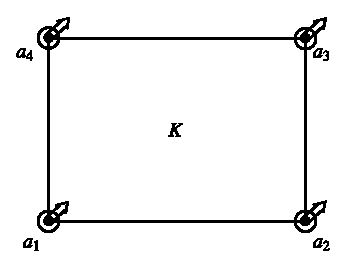
\includegraphics{figure/fig10.1.eps}
\caption{}\label{chap10-fig10.1}
\end{figure}

Equivalently, one may also use the $P_{K}$-unisolvent set
\begin{equation*}
\begin{split}
\sum'_{K}&= \big\{
p(a_{i}),Dp(a_{i})(a_{i+1}-a_{i}),Dp(a_{i})(a_{i-1}-a_{i}),\\
&\quad D^{2}p(a_{i})(a_{i+1}-a_{i},a_{i-1}-a_{i});\ 1\leq i\leq 4\big\}
\end{split}\tag{10.5}\label{chap10-eq10.5}
\end{equation*}
(all\pageoriginale indices being read modulo 4).

Recall that for an affine family of finite elements, the degrees of
freedom $p(a^{0}_{i})$, $Dp(a^{1}_{i})(\xi^{1}_{ik})$,
$(D^{2}p(a^{2}_{i})(\xi^{2}_{ik},\xi^{2}_{il})$ are such that (cf.\@
Sec.~\ref{chap5}): 
\begin{equation*}
\begin{cases}
a^{0}_{i}=F(\hat{a}^{0}_{i}),\ldots,a^{2}_{i}=F(\hat{a}^{2}_{i}),\\
\xi^{1}_{i,k}=B_{K}\hat{\xi}^{1}_{i,k},\ldots,\xi^{2}_{i,1}=B_{K}\hat{\xi}^{2}_{i,1} 
\end{cases}\tag{10.6}\label{chap10-eq10.6}
\end{equation*}
for then $\widehat{\pi_{K}v}=\hat{\pi}\hat{v}$ which is essentially
what we need for the abstract error analysis.

In $\sum'_{K}$ note that
\begin{equation*}
a_{i+1}-a_{i}=F(\hat{a}_{i+1})-F(\hat{a}_{i})=B_{K}(\hat{a}_{i+1}-\hat{a}_{i}),\tag{10.7}\label{chap10-eq10.7} 
\end{equation*}
and so on. Thus it is clear that this rectangle can be imbedded in an
affine family of finite elements. Now $P_{K}\subset \hat{P}\subset
Q_{3}$ for $k=3$. By our abstract error analysis, we therefore have
\begin{equation*}
||u-u_{h}||_{2,\Omega}\leq
Ch^{2}|u|_{4,\Omega}.\tag{10.8}\label{chap10-eq10.8} 
\end{equation*}
assuming sufficient smoothness on $u$ as usual.


A word about the boundary conditions. As in Exercise
\ref{chap3-exer3.1}, we get that $V_{h}\subset H^{2}_{0}(\Omega)$ if
$v=\dfrac{\p v}{\p \nu}=0$ on $\Gamma$, for $v\in V_{h}$. Thus in
choosing our basis functions we must assure ourselves that this
condition is satisfied. This in turn depends on the values at the
boundary nodes. Let $b$ and $c$ be two nodes on $\Gamma$ such that the
line joining them is parallel to (say) the $x_{1}$-axis. Since we need
$v=0$ on this line, and since $v$ will be a polynomial in $x_{1}$ of
degree $\leq 3$ on this line we must have $v(b)=v(c)=0$, $\dfrac{\p
  v}{\p x_{1}}(b)=\dfrac{\p v}{\p x_{1}}(c)=0$. Also since we need
$\dfrac{\p v}{\p \nu}=0$ on this line and since $\dfrac{\p v}{\p
  \nu}=\dfrac{\p v}{\p x_{2}}$ is a polynomial in $x_{1}$ of degree
$\leq 3$, we need to set $\dfrac{\p v}{\p x_{2}}(b)=\dfrac{\p v}{\p
  x_{2}}(c)=0$ and $\dfrac{\p^{2}v}{\p x_{1}\p
  x_{2}}(b)=\dfrac{\p^{2}v}{\p x,\p x_{2}}(c)=0$. Thus the degrees of
freedom\pageoriginale on all boundary nodes must be zero. The only
``free'' or ``unknown'' parameters are the degrees of freedom at the
interior nodes. This takes care of the boundary conditions.
\end{example}

Let us now turn to the {\em Argyris triangle} (cf.\@
Example~\ref{chap4-exam4.7}). 
\begin{figure}[H]
\centering
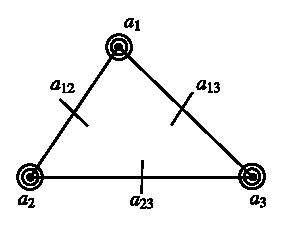
\includegraphics[scale=1.2]{figure/fig10.2.eps}
\caption{}\label{chap10-fig10.2}
\end{figure}

We recall that $P_{K}=P_{5}$, $\dim P_{K}=21$, and $\sum_{K}$ is given
by (cf.\@ Fig.~\ref{chap10-fig10.2})
\begin{equation*}
\sum_{K}=\left\{p(a_{i}),\frac{\p p}{\p
  x_{1}}(a_{i}),\ldots,\frac{\p^{3}p}{\p x^{2}_{2}}(a_{i}), 1\leq
i\leq 3; \frac{\p p}{\p \nu}(a_{ij}),1\leq i<j\leq
3\right\}.\tag{10.9}\label{chap10-eq10.9} 
\end{equation*}

We may replace the first and second derivative values at the vertices
by $Dp(a_{i})(a_{i+1}-a_{i})$, $Dp(a_{i})(a_{i-1}-a_{i})$,
$D^{2}p(a_{i})(a_{i+1}-a_{i},a_{i+1}-a_{i})$,
$D^{2}p(a_{i})(a_{i+1}-a_{i},a_{i-1}-a_{i})$,
$D^{2}p(a_{i})(a_{i-1}-a_{i},a_{i-1}-a_{i})$ in order to get degrees
of freedom for which the relations of the type \eqref{chap10-eq10.6}
may be satisfied. However, {\em one cannot replace the normal
  derivatives $\dfrac{\p p}{\p \nu}(a_{ij})$, $1\leq i<j\leq 3$, by
  such quantities since affine transformations do not preserve
  orthogonality.}

In order to estimate the errors we describe an ``intermediary'' finite
element:

\begin{example}\label{chap10-exam10.2}
The Hermite Triangle of Type (5).

Let $P_{K}=P_{5}(\dim P_{K}=21)$. Define 
\begin{align*}
\sum_{K} &= \Big\{ p(a_{i}),
Dp(a_{i})(a_{i+1}-a_{i}),Dp(a_{i})(a_{i-1}-a_{i}),\\
&\quad D^{2}p(a_{i})(a_{i+1}-a_{i},a_{i+1}-a_{i}),
D^{2}p(a_{i})(a_{i+1}-a_{i},a_{i-1}-a_{i}),\\ 
&\quad D^{2}p(a_{i})(a_{i-1}-a_{i},a_{i-1}-a_{i}),1\leq i\leq 3;\\
&\quad Dp(a_{ij})(a_{k}-a_{ij}), 1\leq i<j\leq 3, k\neq 1, \neq j\Big\}.
\end{align*}\pageoriginale

That is to say, the only change compared to the Argyris triangle is
that we have replaced the normal derivatives at $a_{ij}$ by the
derivatives along the line joining $a_{ij}$ to $a_{k}$, the opposite
vertex.

Symbolically we can represent such a triangle as in
Fig.~\ref{chap10-fig10.3}. 
\begin{figure}[H]
\centering
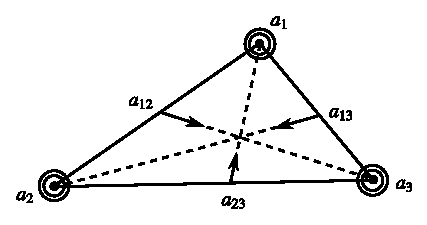
\includegraphics{figure/fig10.3.eps}
\caption{}\label{chap10-fig10.3}
\end{figure}

This element can be put in an affine family as is readily seen. If
$\Lambda_{K}$ is the associated interpolation operator, our error
analysis yields
\begin{equation*}
|v-\Lambda_{K}v|_{m,K}\leq
C\frac{h^{6}_{K}}{\rho^{m}_{K}}|v|_{6,K},\ 0\leq m\leq
6,\tag{10.10}\label{chap10-eq10.10} 
\end{equation*}
for $v\in H^{6}(K)$.
\end{example}

\begin{remark}\label{chap10-rem10.2}
Though the Hermite triangle of type (5) yields an affine family, one
cannot use it since $V_{h}\subset C^{0}(\overline{\Omega})$ but, in
general, $V_{h}\not\subset C^{1}(\overline{\Omega})$ as is necessary
for fourth-order problems. This is so because the adjacent triangles
will not patch up, in general, in their derivatives along the medians;
cf.~\ref{chap10-fig10.4}. 
\end{remark}

\begin{figure}[H]
\centering
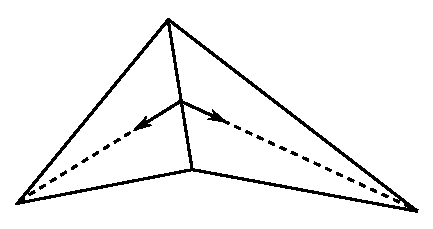
\includegraphics{figure/fig10.4.eps}
\caption{}\label{chap10-fig10.4}
\end{figure}\pageoriginale

Again we show how to take care of the boundary conditions in the
Argyris triangle. We need again $v=\dfrac{\p v}{\p \nu}=0$ on
$\Gamma$. Let us have two nodes $b$, $b'$, the vertices of a triangle
lying on $\Gamma$ with mid-point $c$. On this line $v$ will be a
polynomial of degree $\leq 5$ in $\tau$, an abscissa along this
line. $\dfrac{\p v}{\p \nu}$ will be a polynomial in $\tau$ of degree
$\leq 4$ on this line. Hence for $v=0$ on $\Gamma$ we need to set,
$v(b)=v(b')=0$, $\dfrac{\p v}{\p \tau}(b)=\dfrac{\p v}{\p
  \tau}(b')=0$, $\dfrac{\p^{2}v}{\p \tau^{2}}(b)=\dfrac{\p^{2}v}{\p
  \tau^{2}}(b')=0$. For $\dfrac{\p v}{\p \nu}=0$ on $\Gamma$ we set,
$\dfrac{\p v}{\p \nu}(b)=\dfrac{\p v}{\p \nu}(b')=\dfrac{\p v}{\p
  \nu}(c)=0$, $\dfrac{\p^{2}v}{\p \tau\p \nu}(b)=\dfrac{\p^{2}v}{\p
  \tau \p \nu}(b')=0$. Thus the only free or unknown parameters are
$\dfrac{\p^{2}v}{\p \nu^{2}}$ at vertices on $\Gamma$ and the degrees
of freedom at all interior nodes.

We now get an error estimate when we have triangulations of Argyris
triangles. We use our usual terminology more loosely
here\footnote[1]{Because we have to drop the assumption that all the
  finite elements are affine equivalent to a reference finite
  element.}. By a {\em regular family} of triangulations made up of
Argyris triangles we mean that all $\mathfrak{t}_{h}$ consist only of
Argyris triangles and that for all $K$, $\dfrac{h_{K}}{\rho_{K}}\leq
\sigma$, a constant. We also assume that if
$h=\max\limits_{K\in\mathfrak{t}_{h}}h_{K}$, then $h\to 0$.

\begin{theorem}\label{chap10-thm10.1}
For a regular family $(\mathfrak{t}_{h})$ of triangulations made up of
Argyris triangles
\begin{equation*}
|v-\pi_{h}v|_{m,\Omega}\leq C\ h^{6-m}|v|_{6,\Omega},0\leq m\leq 6.\tag{10.11}\label{chap10-eq10.11}
\end{equation*}\pageoriginale
\end{theorem}

\begin{proof}
Let us denote the opposite vertex of $a_{ij}(i<j)$ by $a_{k}$. Let
$\overrightarrow{\nu}_{_{K}}$ be the unit outernormal at $a_{ij}$ and
$\overrightarrow{\tau}_{_{K}}$ be the unit vector along the line
$[a_{i},a_{j}]$, at $a_{ij}$ (cf.\@ Fig.~\ref{chap10-fig10.5}). 
\begin{figure}[H]
\centering
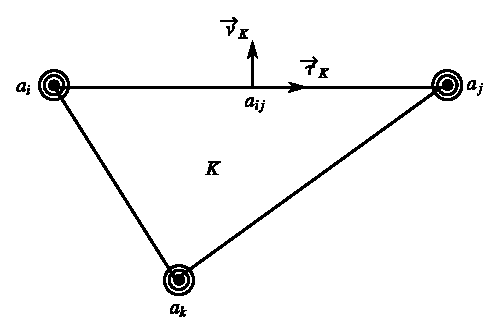
\includegraphics{figure/fig10.5.eps}
\caption{}\label{chap10-fig10.5}
\end{figure}

Let $\pi_{K}$ be the interpolation operator for the Argyris triangle
$K$ and let $\Lambda_{K}$ be that for the corresponding Hermite
triangle of type (5).

Set $\delta=\pi_{K}v-\Lambda_{K}v$. Then $\delta\in P_{5}$. Now
$$
\frac{\p \delta}{\p \nu_{K}}(a_{ij})=\frac{\p}{\p
  \nu_{K}}(\pi_{K}v-\Lambda_{K}v)(a_{ij})=\frac{\p}{\p
  \nu_{K}}(v-\Lambda_{K}v)(a_{ij}). 
$$

Also since $\pi_{K}v=\Lambda_{K}v$ along any side of $K$ (since the
values of these polynomials of degree 5 as well as those of their
first and second derivatives agree at the end-points), we have
$\dfrac{\p \delta}{\p \tau_{K}}=0$.

Since
$$
D\delta (a_{ij})(a_{k}-a_{ij})=\frac{\p \delta}{\p
  \nu_{K}}(a_{ij})\langle a_{k}-a_{ij},\ora{\nu}_{K}\rangle+\frac{\p
  \delta}{\p \tau_{K}}(a_{ij})\langle
a_{k}-a_{ij},\ora{\tau}_{K}\rangle, 
$$
where $\langle \cdot,\cdot\rangle$ is the Euclidean inner-product,
substituting for $\dfrac{\p \delta}{\p \nu_{K}}$ and $\dfrac{\p
  \delta}{\p \tau_{K}}$ at $a_{ij}$, we get
\begin{equation*}
D\delta (a_{ij})(a_{k}-a_{ij})=\frac{\p}{\p
  \nu}(v-\Lambda_{K}v)(a_{ij})\langle
a_{k}-a_{ij},\ora{\nu}_{K}\rangle\tag{10.12}\label{chap10-eq10.12} 
\end{equation*}

Since\pageoriginale $\delta\in P_{5}$, using the unisolvency in the
Hermite triangle we may express $\delta$ in terms of its basis
functions. Since all degrees of freedom except those of the type
$D\delta(a_{ij})(a_{k}-a_{ij})$ are zero for $\delta$, we have
\begin{equation*}
\delta=\sum_{\substack{1\leq i<j\leq 3\\ k\neq i, k\neq
    j}}\frac{\p}{\p \nu_{K}}(v-\Lambda_{K}v)(a_{ij})\langle
a_{k}-a_{ij},\ora{\nu}_{K}\rangle p_{ijk}.\tag{10.13}\label{chap10-eq10.13}
\end{equation*}

Now 
\begin{equation*}
|\langle a_{k}-a_{ij},\ora{\nu}_{K}\rangle |\leq
||a_{k}-a_{ij}||~||\ora{\nu}_{K}||\leq h_{K},\tag{10.14}\label{chap10-eq10.14}
\end{equation*}
and
\begin{align*}
|\frac{\p}{\p \nu_{K}}(v-\Lambda_{K}v)(a_{ij})| &\leq
|v-\Lambda_{K}v|_{1,\infty,K}\\ 
&\leq C(\meas K)^{-\frac{1}{2}}\frac{h^{6}_{K}}{\rho_{K}}|v|_{6,K}. 
\end{align*}
(Theorem \ref{chap6-thm6.6} with $m=1$, $k=5$, $p=2$,
$q=\infty$). Also, $\meas K\geq C\rho^{2}_{K}$, and we have
\begin{equation*}
|\frac{\p}{\p \nu_{K}}(v-\Lambda_{K}v)(a_{ij})|\leq
C\frac{h^{6}_{K}}{\rho^{2}_{K}}|v|_{6,K}.\tag{10.15}\label{chap10-eq10.15} 
\end{equation*}

Finally, by Theorem \ref{chap6-thm6.4} and \ref{chap6-thm6.5}
\begin{equation*}
|p_{ijk}|_{m,K}\leq
C\frac{h_{K}}{\rho^{m}_{K}}|\hat{p}_{ijk}|_{m,\hat{K}}.\tag{10.16}\label{chap10-eq10.16} 
\end{equation*}

Combining \eqref{chap10-eq10.14}, \eqref{chap10-eq10.15} and
\eqref{chap10-eq10.16}, we get
\begin{align*}
|\delta|_{m,K} &\leq \sum_{\substack{1\leq i<j\leq 3\\ k\neq i, k\neq
    j}} |\frac{\p}{\p \nu_{K}}(v-\Lambda_{K}v)(a_{ij})|~|\langle
a_{k}-a_{ij},\ora{\nu}_{K}\rangle|~|p_{ijk}|_{m,K}\\
&\leq C\frac{h^{8}_{K}}{\rho^{m+2}_{K}}|v|_{6,K},
\tag{10.17}\label{chap10-eq10.17} 
\end{align*}
and hence, 
\begin{align*}
|v-\pi_{K}v|_{m,K} &\leq |v-\Lambda_{K}v|_{m,K}+|\delta|_{m,K}\\
&\leq
C\frac{h^{6}_{K}}{\rho^{m}_{K}}\left(1+\frac{h^{2}_{K}}{\rho^{2}_{K}}\right)|v|_{6,K}\quad\text{(Using
  \eqref{chap10-eq10.10} and \eqref{chap10-eq10.17})}\\
&\leq C\ h^{6-m}|v|_{6,K}\quad(\text{since~ } h_{K}\leq h,
\frac{h_{K}}{\rho_{K}}\leq \sigma). 
\end{align*}\pageoriginale

This on summing over $K$ gives \eqref{chap10-eq10.11}, thus completing
the proof.
\end{proof}

\begin{exercise}\label{chap10-exer10.1}
Perform the same analysis for the 18-degree-of freedom
triangle. (cf.\@ Exercise \ref{chap4-exer4.7}).
\end{exercise}

For the interpolation theory of the HCT-triangle (cf.\@ Exercise
\ref{chap4-exer4.8}), the normal derivatives are handled as in the
present case. However the arbitrariness of the interior point is an
obstacle to be overcome. For a discussion of this, see Ciarlet
\cite{key4}. 

Another finite element, similar in its principle to the HCT-triangle
used in the conforming finite element method for the plate problem is
the {\em Fraeijs} de Veubeke and Sander Quadrilateral. See Ciavaldini
and N\'ed\'elec \cite{key9}.

These are all essentially the finite elements used in the
``conforming'' methods to approximate the plate problem (we will
define such methods at the beginning of Sec.~\ref{chap11}).








